% arara: pdflatex: { shell: yes }
% arara: biber
% arara: pdflatex: { shell: yes }
% arara: pdflatex: { shell: yes }

% Demo report and presentation prepared by Aaron English (humdrumcomet on github)
\documentclass[hidelinks, 12pt]{article}%

\usepackage{geometry} % useful for defining page geometries
\usepackage{hyperref} % used for creating hyperlinks in documents. Both to the web and within the document itself
\usepackage[tbtags]{amsmath} % for typesetting math (American Mathematical Society)
\usepackage{amsfonts} % fonts and mathematical symbols
\usepackage{amssymb} % more mathematical symbols
\usepackage[utf8]{inputenc} % how to treat the written file (as utf8)
\usepackage[T1]{fontenc} % the encoding for the output file T1 is the most common, includes accents and many other commonly needed/used characters
\usepackage[style=ieee,backend=biber]{biblatex} % for handling bibliographies
\usepackage{float} % added control over
\usepackage{graphicx} % tools for inclusion of graphics
\usepackage{booktabs} % adding commands to improve the look of tables
\usepackage{csvsimple} % simplify table creation by importing .csv files directly
\usepackage{siunitx} % consistent notation and correct formatting of units
\DeclareSIUnit{\torr}{Torr} % Custom unit definition
\usepackage{minted} % inclusion of code blocks with syntax highlighting and
\setminted{linenos, autogobble, fontsize=\footnotesize, breaklines=true} % set global options for minted environments
\usepackage{chemformula} % for writing chemical formulae
\usepackage[useregional]{datetime2}
\usepackage{enumitem}
\usepackage{appendix}
\usepackage{caption}
\usepackage{listings}
\usepackage{xstring}
\usepackage{titlesec}
\usepackage{titlecaps}
\addbibresource[location=local]{references.bib} % adding a bibliography

 \renewcommand{\thesubsubsection}{\thesubsection\hspace{5pt}\alph{subsubsection}}

\newcommand{\round}[1]{\tablenum[exponent-mode=scientific, round-precision=4,
        round-mode=places, table-format=1.3e1]{#1}}

\newcommand{\roundformation}[1]{\tablenum[exponent-mode=scientific, round-precision=3,
        round-mode=places, table-format=1.3e1]{#1}}

\renewcommand{\lstlistingname}{Code Attachment}% Listing -> Algorithm
\renewcommand{\lstlistlistingname}{List of \texttt{MATLAB} \lstlistingname s}% List of Listings -> List of Algorithms   

% \setcounter{secnumdepth}{4}
% \titleformat{\paragraph}
% {\normalfont\normalsize\bfseries}{\theparagraph}{1em}{}
% \titlespacing*{\paragraph}
% {0pt}{3.25ex plus 1ex minus .2ex}{1.5ex plus .2ex}
% % \renewcommand{\theparagraph}{\thesubsection\hspace{5pt}\alph{subsubsection}\hspace{5pt}\roman{paragraph}}
\titleclass{\subsubsubsection}{straight}[\subsection]

\newcounter{subsubsubsection}[subsubsection]
\renewcommand\thesubsubsubsection{\thesubsubsection.\arabic{subsubsubsection}}
\renewcommand\theparagraph{\thesubsubsubsection.\arabic{paragraph}} % optional; useful if paragraphs are to be numbered

\titleformat{\subsubsubsection}
  {\normalfont\normalsize\bfseries}{\thesubsubsubsection}{1em}{}
\titlespacing*{\subsubsubsection}
{0pt}{3.25ex plus 1ex minus .2ex}{1.5ex plus .2ex}

\makeatletter
\renewcommand\paragraph{\@startsection{paragraph}{5}{\z@}%
  {3.25ex \@plus1ex \@minus.2ex}%
  {-1em}%
  {\normalfont\normalsize\bfseries}}
\renewcommand\subparagraph{\@startsection{subparagraph}{6}{\parindent}%
  {3.25ex \@plus1ex \@minus .2ex}%
  {-1em}%
  {\normalfont\normalsize\bfseries}}
\def\toclevel@subsubsubsection{4}
\def\toclevel@paragraph{5}
\def\toclevel@paragraph{6}
\def\l@subsubsubsection{\@dottedtocline{4}{7em}{4em}}
\def\l@paragraph{\@dottedtocline{5}{10em}{5em}}
\def\l@subparagraph{\@dottedtocline{6}{14em}{6em}}
\makeatother

\setcounter{secnumdepth}{4}
\setcounter{tocdepth}{4}


\renewcommand{\thesubsubsubsection}{\thesubsection\hspace{5pt}\alph{subsubsection}\hspace{5pt}\roman{subsubsubsection}}


\begin{document}
    \setcounter{page}{0}
    \begin{center}
        \vspace*{1cm}
        {\fontsize{300}{50}\selectfont {\bfseries AERO 3240 Term Assignment\\}}
        \vspace{3cm}
        {\LARGE Carleton University \\}
        \vspace{8cm}
    \end{center}
    \begin{center}
        By: 
        Boaz Aharony\\ \vspace{10pt}
        Student ID: 
        REDACTED\\ \vspace{10pt}
        \DTMdisplaydate{2022}{12}{7}\\
    \end{center}
    \thispagestyle{empty}

    \clearpage

    \section*{Notes}
    All figures, code attachments, tables, code lines, and section references are clickable and will bring you to said reference. As well all 2-D plots are vectored images that allow unlimited zoom-in.
    
    \tableofcontents
    
    \clearpage
    
    \listoffigures
    \listoftables
    \lstlistoflistings
    
    \clearpage
    


\setcounter{section}{1}
    \section{Two-Body Problem}
    
    \setcounter{subsection}{4}
    \subsection{Speed and Periods of Circular LEO}
    \label{question 2.5}
Created using code attachment \ref{2.5 script} in Appendix \ref{2.5 appendix}.
\begin{figure}[H]
    \begin{centering}
        \includegraphics[width=\textwidth]{output_files/2.5/Orbit_Altitude_vs_Velocity.eps}
        \caption{Orbital Speed vs Altitude}
        \label{2.5 altitude vs speed circular LEO}
    \end{centering}
\end{figure}
    
\begin{figure}[H]
    \begin{centering}
        \includegraphics[width=\textwidth]{output_files/2.5/Orbit_Altitude_vs_period.eps}
        \caption{Orbital Period vs Altitude}
        \label{2.5 altitude vs period circular LEO}
    \end{centering}
\end{figure}
        
\setcounter{subsection}{12}
\subsection{PROBA-2 Without Perturbations}
\label{question 2.13}
Created using \texttt{MATLAB} code and \texttt{SIMULINK} diagrams found in Appendix \ref{2.13 appendix}.

\subsubsection{Plot of Orbit in the Orbital Plane}
Created using code attachment \ref{2.13 script} after line \ref{line: 2.13 part A}
\begin{figure}[H]
    \begin{centering}
        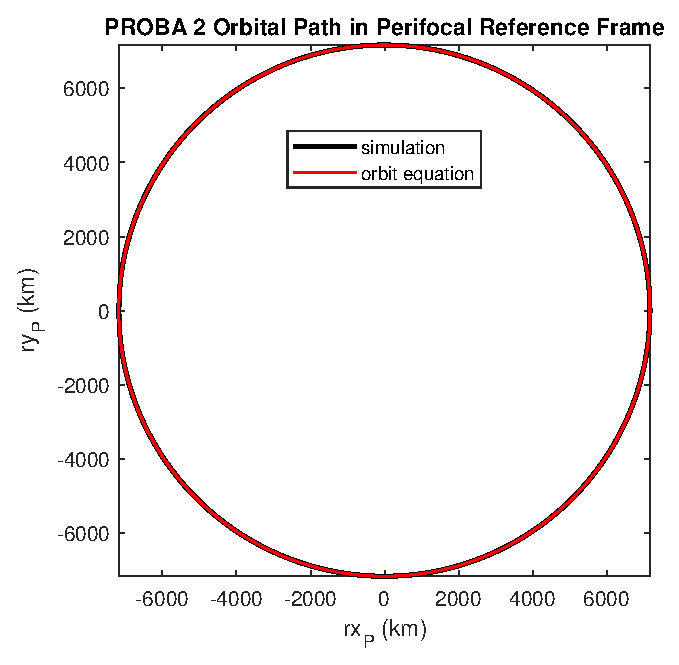
\includegraphics[width=\textwidth]{output_files/2.13/perifocal_plot.eps}
        \caption{PROBA-2 Orbit in Perifocal Frame}
        \label{perifocal 2.13}
    \end{centering}
\end{figure}


\subsubsection{Initial Conditions For \texttt{SIMULINK} Integrators}
Calculated in code attachment \ref{2.13 script} after line \ref{line: 2.13 part B} using rotation matrix functions found in appendix \ref{appendix: rotation matrices}
%TODO ask if to add explanation of rotation matrices
\begin{table}[H]
    \centering
    \caption{Table of Initial PROBA-2 Position and Velocity}
    \vspace{0.1cm}
    \csvreader[
        head to column names,
        tabular = ccc,
        table head = \toprule \bfseries Component & \bfseries $\mathbf{r}_{I,initial}$(km) & \bfseries 
        $\mathbf{v}_{I,initial}$(km/s) \\\midrule,
        table foot = \bottomrule,
        ]{output_files/2.13/initial_conditions.csv}{}{\csvcoli & \round{\csvcolii} & \round{\csvcoliii}}
    \label{Table:Parameters}

\end{table}
        
\subsubsection{3D plot of Orbit}
An animation of one orbit cycle can be viewed by clicking this 
\href{https://youtu.be/kpSWNcpdS9Y}{\textbf{\textcolor{blue}{youtube link}}} (done using attachment \ref{video animation 3d orbit}, does not show earth's spin)\\[5pt]
The figure below was created using code attachment \ref{2.13 script} after line \ref{line: 2.13 part C}
\begin{figure}[H]
    \begin{centering}
        \includegraphics[width=\textwidth]{output_files/2.13/3d_plot.png}
        \caption{3-D Plot of PROBA-2 Orbit Around Earth}
        \label{3d 2.13}
    \end{centering}
\end{figure}


\subsubsection{Components of Position and Velocity in ECIF}
Created using code attachment \ref{2.13 script} after line \ref{line: 2.13 part D}
\begin{figure}[H]
    \begin{centering}
        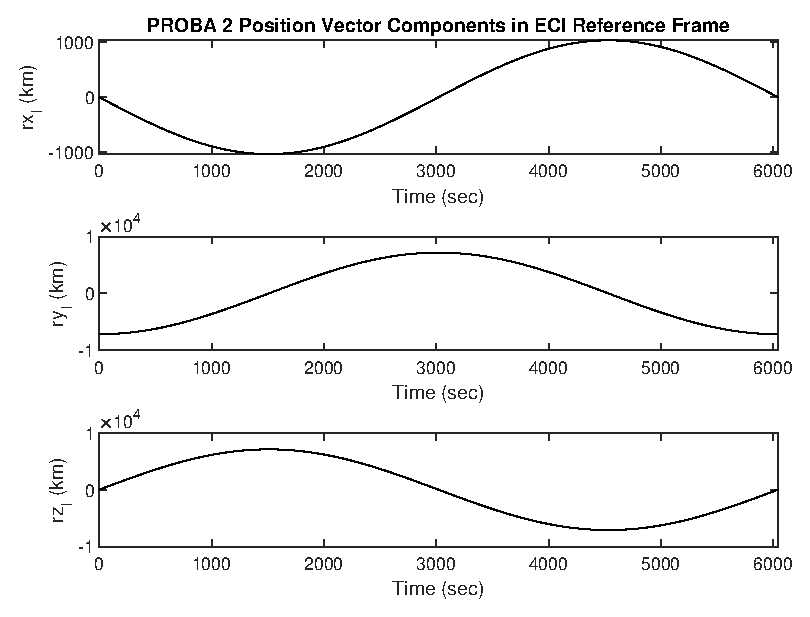
\includegraphics[width=\textwidth]{output_files/2.13/position_components.eps}
        \caption{PROBA-2 Components of Position}
        \label{position components 2.13}
    \end{centering}
\end{figure}

\begin{figure}[H]
    \begin{centering}
        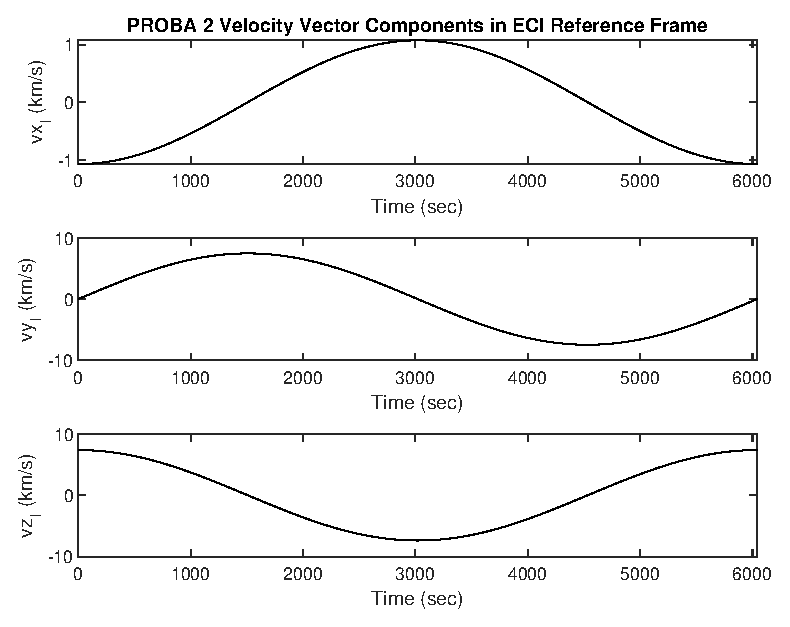
\includegraphics[width=\textwidth]{output_files/2.13/velocity_components.eps}
        \caption{PROBA-2 Components of Velocity}
        \label{velocity components 2.13}
    \end{centering}
\end{figure}

\subsubsection{Radius and Speed in ECIF}
Created using code attachment \ref{2.13 script} after line \ref{line: 2.13 part E}
\begin{figure}[H]
    \begin{centering}
        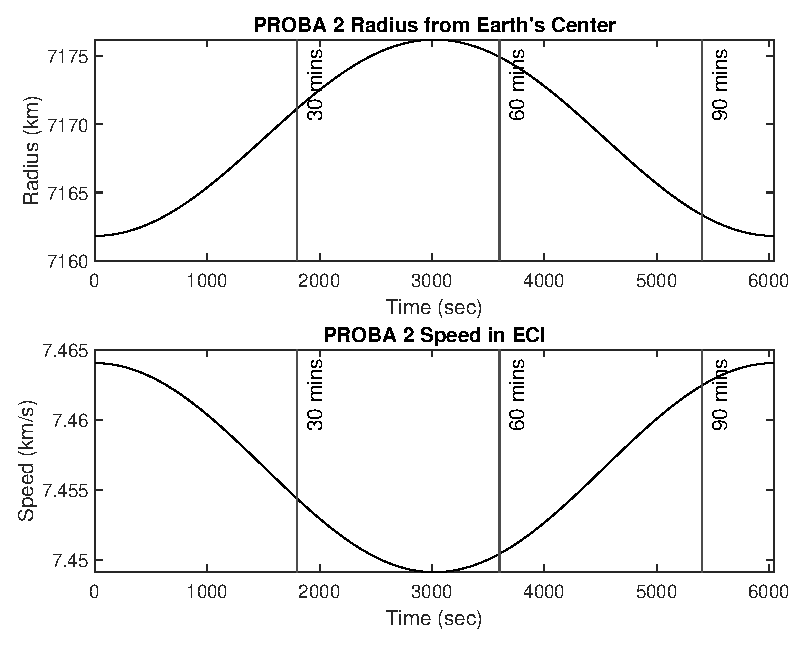
\includegraphics[width=\textwidth]{output_files/2.13/radius_and_speed.eps}
        \caption{PROBA-2 Radius and Speed}
        \label{radius and speed 2.13}
    \end{centering}
\end{figure}

Using the Vis-Viva equation as a function of radius $r$ for a constant semi-major axis $a$ the velocity at any point is determined by eq. \ref{eq: vis-viva}
\begin{equation}
    v = \sqrt{\mu\left(\frac{2}{r}-\frac{1}{a}\right)}
    \label{eq: vis-viva}
\end{equation}
The radius was determined in code by finding the position in the array of the closest time point and taking its radius, which was visually compared with the above graphs. To verify the graphs, the results compared to eq. \ref{eq: vis-viva} are confirmed in table \ref{Table:vis_viva}:


\begin{table}[H]
    \centering
    \caption{Table of comparison between simulation and vis-viva results}
    \vspace{0.1cm}
    \csvreader[
        head to column names,
        tabular = cccc,
        table head = \toprule \bfseries Time (minutes) & \bfseries $\mathbf{r}_{I}$(km) & \bfseries 
        Calculated $\mathbf{v}_{I}$(km/s) & \bfseries Simulated $\mathbf{v}_{I}$(km/s)\\\midrule,
        table foot = \bottomrule,
        ]{output_files/2.13/vis_viva_check.csv}{}{\csvcoli & \round{\csvcolii} & \round{\csvcoliii} & \round{\csvcoliv}}
    \label{Table:vis_viva}

\end{table}

\subsubsection{Ground Plots}

Video animated ground tracks are available by clicking this \href{https://youtu.be/-6w7wiyfnvI}{\textbf{\textcolor{blue}{youtube link}}} (done using attachment \ref{video animation ground tracks}) As well as the plot below which was created using code attachment \ref{2.13 script} after line \ref{line: 2.13 part F}:
\begin{figure}[H]
    \begin{centering}
        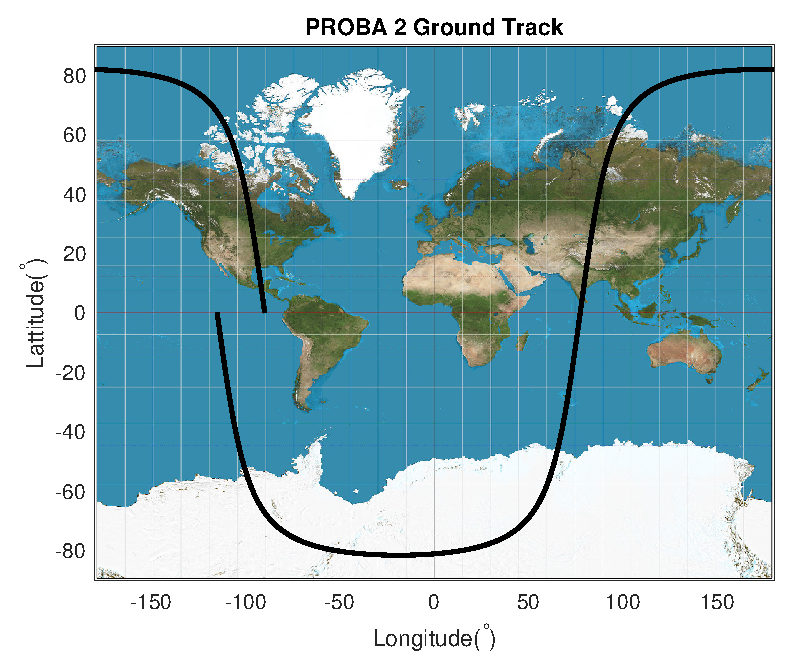
\includegraphics[width=\textwidth]{output_files/2.13/ground_tracks.eps}
        \caption{PROBA-2 ground tracks}
        \label{ground tracks 2.13}
    \end{centering}
\end{figure}



\section{Orbital Pertubations}
\subsection{PROBA-2 with Pertubations}
\label{question 3.1}
Created using \texttt{MATLAB} code and \texttt{SIMULINK} diagrams found in Appendix \ref{3.1 appendix}.

\subsubsection{Calculated Secular and Average Rate of Change}
To determine the expected secular change in RAAN eq. \ref{eq: secular change in RAAN} is used
\begin{equation}
    \Delta\Omega =-\frac{3\pi J_2 R_{\oplus}^{2}}{p^2}\cos{(i)}
    \label{eq: secular change in RAAN}
\end{equation}

\noindent To determine the expected average rate of change eq. \ref{eq: average change in RAAN} is used:
\begin{equation}
    \langle\dot\Omega\rangle=-\frac{3 J_2 R_{\oplus}^{2}}{2p^2}n\cos{(i)}
    \label{eq: average change in RAAN}
\end{equation}

\noindent This is calculated in section A of \texttt{MATLAB} code attachment \ref{3.1 script} after line \ref{line: 3.1 part A}. It is tabulated in Tables \ref{Table: RAAN 98.28} and \ref{Table: RAAN 10} for inclinations of $98.28^{\circ}$ and $10^{\circ}$ respectively. These tables are found in \ref{comparison 3.1}.

\subsubsection{Simulating with $\text{J}_2$}
The simulation was done by adding the $J_2$ perturbation function in code attachment \ref{J_2 function for 3.1} to the \texttt{SIMULINK} diagram Figure \ref{3.1 diagram} as a function block and summation with the acceleration caused by the two-body-problem. The main script attachment \ref{3.1 script} uses the simulation for the rest of the question.

\subsubsection{Plot of Change in RAAN}
Done in code attachment \ref{3.1 script} after line \ref{line: 3.1 part C}
\label{change in raan 3.1}
\foreach \i in {98.28,10}{
\begin{figure}[H]
    \begin{centering}
        \includegraphics[width=\textwidth]{output_files/3.1/RAAN_\i_degrees.eps}
        \caption{PROBA-2 Change in RAAN at $\i^\circ$  inclination}
        \label{fig: RAAN 3.1 at \i}
    \end{centering}
\end{figure}
}


\subsubsection{Interpretation of Change in RAAN from Simulation}
Calculated after line \ref{line: 3.1 part D} of \texttt{MATLAB} code attachment \ref{3.1 script} and tabulated in Tables \ref{Table: RAAN 98.28} and \ref{Table: RAAN 10} for inclinations of $98.28^{\circ}$ and $10^{\circ}$ respectively. These tables are found in \ref{comparison 3.1}.

\subsubsection{Comparison of Expected and Simulated Secular and Rate of Change in RAAN}
\label{comparison 3.1}
Done in code attachment \ref{3.1 script} after line \ref{line: 3.1 part E}

\foreach \i in {98.28,10}{
\begin{table}[H]
    \centering
    \caption{Table of comparison between simulation and calculated RAAN results for inclination of $\i^{\circ}$}
    \vspace{0.1cm}
    \csvreader[
        head to column names,
        tabular = ccc,
        table head = \toprule  & \bfseries secular change ($^{\circ}$/rev) & \bfseries 
        average rate of change($^{\circ}$/s)\\\midrule,
        table foot = \bottomrule,
        ]{output_files/3.1/RAAN_check_for_inc_\i.csv}{}{
        \bfseries \csvcoli & \round{\csvcolii} & \round{\csvcoliii}
        }
    \label{Table: RAAN \i}
\end{table}
}



\subsubsection{Repeat for $10^{\circ}$ Inclination}
The repeat is done in Figure \ref{fig: RAAN 3.1 at 10} and Table \ref{Table: RAAN 10} by changing the initial i (inclination) value in code attachment \ref{3.1 script} on line \ref{line: 3.1 inclination val}.

\setcounter{section}{4}
\section{Spacecraft Formation Flying }
\subsection{Envisat Formation}
\label{question 5.1}
\setcounter{subsubsection}{5}
\subsubsection{Confirmation of Answers with \texttt{MATLAB}}
Created using code attached in Appendix \ref{5.1 Appendix}\\[5pt]

% % initial conditions for each graph
% \newcommand{\eqalongtrack}{
% For $\SI{10}{\kilo \meter}$ separation along-track formation:\\
% $x_0 = \dot x_o=z_0 = \dot z_0=\dot y_0 = 0$\\
% and:\\
% $y_0 = \SI{10}{\kilo \meter}$
% }
% \newcommand{\eqintrack}{
% For $\SI{10}{\kilo \meter}$ along-track separation for an in-track formation:\\
% $x_0 = \dot x_o= \dot z_0=\dot y_0 = 0$\\
% and:\\
% $y_0 = \SI{10}{\kilo \meter}$\\
% $z_0$ can be calculated using eq. \ref{eq: z_0 in track}
% \begin{equation}
%     z_0 = -\left(\frac{\omega_\oplus}{n}\sin i\right)y_0
%     \label{eq: z_0 in track}
% \end{equation}
% This works out to approximately:\\
% $z_0 = \SI{-0.6899}{\kilo \meter}$
% }

% \newcommand{\eqinplaneeliptical}{
% For in-plane elliptical formation with a semi-major axis of $\SI{0.5}{\kilo \meter}$:\\
% $x_0 = \dot x_o= \dot z_0=\dot y_0 = 0$\\
% and:\\
% $y_0 = \SI{10}{\kilo \meter}$\\
% $z_0$ can be calculated using eq. \ref{eq: z_0 in track}
% \begin{equation}
%     z_0 = -\left(\frac{\omega_\oplus}{n}\sin i\right)y_0
%     \label{eq: z_0 in track}
% \end{equation}
% This works out to approximately:\\
% $z_0 = \SI{-0.6899}{\kilo \meter}$
% }
% finish this



\foreach \i\k in {1/(along-track formation),2/(in-track formation),3/(in-plane elliptical formation),4/(circular formation),5/(projected circular formation)}{
\StrSubstitute{\k}{(}{}[\tempa]
\StrSubstitute{\tempa}{)}{}[\tempb]
\subsubsubsection{\titlecap{\tempb}}
Initial conditions in table \ref{Table: formation initial conditions \i} are calculated in code attachment \ref{5.1 script} after line \ref{line: 5.1 case \i}.\\
% For in plane eliptical
\ifnum \i=3
Assuming initial phase angle $\alpha = 0$ for initial conditions in table \ref{Table: formation initial conditions \i}.
\fi  
 

\newcommand{\kms}{\left(\frac{\text{km}}{\text{s}}\right)}
\begin{table}[H]
    \centering
    \caption{Table of initial formation conditions \k}
    \vspace{0.1cm}
    \csvreader[
        head to column names,
        tabular = cccccc,
        table head =  \toprule  $\mathbf{v_{x_0}}\kms$  & $\mathbf{v_{y_0}}\kms$
        &$\mathbf{v_{z_0}}\kms$ & $\mathbf{x_0}$(km) & $\mathbf{y_0}$(km) & $\mathbf{z_0}$(km)\\ \midrule,
        table foot = \bottomrule,
        before reading= \setlength{\tabcolsep}{10pt},
        ]{output_files/5.1/initial_conditions_\i.csv}{}{
         \roundformation{\csvcoli} & \roundformation{\csvcolii} & \roundformation{\csvcoliii} & \roundformation{\csvcoliv} & \roundformation{\csvcolv} & \roundformation{\csvcolvi}
        }
        
    \label{Table: formation initial conditions \i}
\end{table}

\ifnum \i>3
\ifnum \i<6
$\mathbf{z_0}$ and $\mathbf{v_{z_0}}$ in table \ref{Table: formation initial conditions \i} can also be negated and achieve the same formation type.
\fi
\fi

\newcommand{\positiondata}{Position_component_plots_}
\newcommand{\threeDplot}{3D-plot_of_path_around_target_}
\newcommand{\pathinplanes}{Path_in_projected_planes_}

    \foreach \j in {\positiondata,\threeDplot,\pathinplanes}{
        \begin{figure}[H]
            \begin{centering}
                \includegraphics[width=\textwidth,height=0.95\textheight,keepaspectratio]{output_files/5.1/\j\i.eps}
                \StrSubstitute{\j \k}{_}{\space}[\temp]
                \caption{\temp}
                \label{fig: \j}
            \end{centering}
        \end{figure}
       }
}
\clearpage
\appendixtitleon
\appendixtitletocon
\begin{appendices}

\section{\texttt{MATLAB} code for \ref{question 2.5}}
\label{2.5 appendix}

\inputminted{Matlab}{output_files/2.5/AERO_3240_2_5.m}
\captionof{lstlisting}{Script used in question \ref{question 2.5}}
        \label{2.5 script}
            
\section{\texttt{MATLAB} Code for \ref{question 2.13}}
\label{2.13 appendix}
\subsection{General Script}

\inputminted[mathescape=true]{Matlab}{output_files/2.13/PROBA2.m}
\captionof{lstlisting}{Script used in question \ref{question 2.13} \label{2.13 script}}


\subsection{\texttt{SIMULINK} diagram}
 \begin{figure}[H]
        \begin{centering}
            \includegraphics[width=\textwidth]{output_files/2.13/model_2.13.png}
            \caption{\texttt{SIMULINK} model for question \ref{question 2.13}}
            \label{2.13 diagram}
        \end{centering}
    \end{figure}

\subsection{additional functions}
\subsubsection{TBP function}

\begin{minted}[]{matlab}
function a_I  =  TBP(r_I, mu)
% ---------------------------------------------------------------
% TBP
% ---------------------------------------------------------------
% Description:
% Compute the spacecraft acceleration in ECI, using the two-body
% equation of motion.
% ---------------------------------------------------------------
% Inputs:
% r_I => components of r in ECI (3 x 1 matrix)
% ---------------------------------------------------------------
% Outputs:
% a_I => components of the acceleration in ECI (3 x 1 matrix)
% ---------------------------------------------------------------
% Parameters:
% mu => gravitational constant of the Earth
% ---------------------------------------------------------------
% Copyright:
% Steve Ulrich, 2014 
% ---------------------------------------------------------------

% Compute orbital radius
rmod = sqrt( r_I(1)*r_I(1) + r_I(2)*r_I(2) + r_I(3)*r_I(3) );

% Spacecraft acceleration
a_I = -mu/rmod^3*r_I; 
end
 \end{minted}  
\captionof{lstlisting}{Function to calculate $\text{a}_I$ in 
\texttt{SIMULINK} model\label{2.13 TBP function}}
                
\subsubsection{ECI to ECEF function}
\inputminted[]{Matlab}{output_files/2.13/r_I2r_F.m}
\captionof{lstlisting}{Function used to convert vector from ECIF to ECEF}


\section{\texttt{MATLAB} code for \ref{question 3.1}}
\label{3.1 appendix}
\subsection{general script}
\inputminted[mathescape=true]{Matlab}{output_files/3.1/PROBA2_Chapter3.m}
\captionof{lstlisting}{Script used in question \ref{question 3.1} \label{3.1 script}}

\subsection{\texttt{SIMULINK} diagram}
    \begin{figure}[H]
        \begin{centering}
            \includegraphics[width=\textwidth]{output_files/3.1/model_3.1.png}
            \caption{\texttt{SIMULINK} model for question \ref{question 3.1}}
            \label{3.1 diagram}
        \end{centering}
    \end{figure}
\subsection{additional functions}
Refer to code attachment \ref{2.13 TBP function} for TBP function used in Figure \ref{3.1 diagram}.
\subsubsection{$\text{J}_2$ Perturbation acceleration function}

\begin{minted}{matlab}
function f_J2_I =  J2P(rE, J_2, mu, r_I)

% ---------------------------------------------------------------
% J2P
% ---------------------------------------------------------------
% Description:
% Compute the spacecraft acceleration due to J2 perturbation ECI
% ---------------------------------------------------------------
% Inputs:
% r_I => components of r in ECI (3 x 1 matrix)
% ---------------------------------------------------------------
% Outputs:
% f_J2_I => components of the acceleration in ECI (3 x 1 matrix)
% ---------------------------------------------------------------
% Parameters:
% mu => gravitational constant of the Earth
% J_2 => J2 coefficient for oblate body of earth
% rE => Radius of earth
% ---------------------------------------------------------------

% J_2 equation
f_J2_I = 3*mu*J_2*rE^2/(2*(norm(r_I)^5))...
    *(...
    (5*(r_I(3)^2)/(norm(r_I)^2)-1)*r_I - 2*[0; 0; r_I(3)]...
    );

end
\end{minted}   
\captionof{lstlisting}{Function to calculate $\text{J}_2$ perturbation in \texttt{SIMULINK}}
                \label{J_2 function for 3.1}

                
\section{\texttt{MATLAB} code for \ref{question 5.1}}
\label{5.1 Appendix}
\subsection{Main Script}
 \inputminted[mathescape=true]{Matlab}{output_files/5.1/CWH.m}
        \captionof{lstlisting}{Script used in question \ref{question 5.1} \label{5.1 script}}
\subsection{Additional Functions}
\subsubsection{Hill's Equation function}
 \inputminted[mathescape=true]{Matlab}{output_files/5.1/CWHdyn.m}
        \captionof{lstlisting}{Function used to set up Hill's equation\label{5.1 hills equation}}






\section{General \texttt{MATLAB} Functions}
\subsection{Rotation matrix functions}
    \label{appendix: rotation matrices}
    \subsubsection{rotation around x}
        \inputminted[]{Matlab}{general code/C_1.m}
        \captionof{lstlisting}{Function to generate a rotation matrix around the x axis \label{function rotx}}
\vspace{10pt}
    \subsubsection{rotation around y}
        \inputminted[]{Matlab}{general code/C_2.m}
        \captionof{lstlisting}{Function to generate a rotation matrix around the y axis \label{function roty}}
\vspace{10pt}
    \subsubsection{rotation around z}
        \inputminted[]{Matlab}{general code/C_3.m}
        \captionof{lstlisting}{Function to generate a rotation matrix around the z axis \label{function rotz}}
\subsection{Animation functions}
\subsubsection{Video Animate 3-D orbit}
\inputminted[]{Matlab}{general code/draw_earth.m}
        \captionof{lstlisting}{Script to generate orbit animation video \label{video animation 3d orbit}}
        
\subsubsection{Video Animate ground tracks}
\inputminted[]{Matlab}{general code/draw_tracks.m}
        \captionof{lstlisting}{Script to generate ground tracks animation video \label{video animation ground tracks}}
                   
\end{appendices}
   

\end{document}
